\section{Quantum Models}
\label{sec:quantum_models}

The rationale behind building a quantum version of a Game Theory and/or Statistics problem lays in bringing phenomena like quantum superposition, and entanglement into known frameworks allowing different results, that seemingly perform at least as good as their classical versions.

[To Introduce more SOURCES]

The effort put in converting known classical problems also enables the familiarization with the potential differences these models bring.

\subsection{Quantum Roulette}
\label{subsec:quantum_roulette}

In the arbitrary $N$-State quantum roulette, \cite{} presented a $N$-State roulette model using permutation matrices.
To verify this model with two players we developed a Matlab simulation \ref{simulaMalab}, as proposed by the authors.

The game in represented in a $N$-Dimensional Hilbert Space. There is a basis in the space that represents each of the equally probable entries as shown in \ref{eq:roulette_1}. In a sense this is a generalization of a quantum coin flip that is also used in \ref{subsec:quantum_walk_line}.
\begin{equation}
\label{eq:roulette_1}
\vert1\rangle=\left[\begin{array}{c}
1\\
0\\
0\\
\vdots\\
0
\end{array}\right],\:\vert2\rangle=\left[\begin{array}{c}
0\\
1\\
0\\
\vdots\\
0
\end{array}\right],\:\ldots,\:\vert N\rangle=\left[\begin{array}{c}
0\\
0\\
0\\
\vdots\\
1
\end{array}\right]
\end{equation}

Each state transition is obtained using a permutation matrix denoted by $P^{i}$. There are $N!$ permutation matrices, so in the particular case of having a $3$-State roulette, there are $6$ possible transition choices. The classical strategy considered will rely on choosing an arbitrary probability distribution, that verifies\ref{eq:roulette_2}, and that maps the usage of the permutation matrices. This step will not affect the density matrix ($\rho$) of the roulette\ref{eq:roulette_3}.

\begin{equation}
\label{eq:roulette_3}
\rho=\frac{1}{N!}\sum_{i=0}^{N!-1}P^{i}
\end{equation}

\begin{equation}
\label{eq:roulette_2}
\sum_{i=0}^{N!-1}p_{i}=1
\end{equation}

The density matrix is diagonalizable by a Discrete Fourier Transform because it is a kind of circulant matrix\cite{Davis1994}, as we can see in \ref{eq:roulette_4}. In \ref{eq:roulette_4} $\lambda_{k}$ are eigenvalues of $\rho$. $\lambda_{1}=1$
while $\lambda_{2}=\lambda_{3}=\lambda_{k}=\lambda_{N-1}=0$. Each column
$i$ of the Fourier matrix will represent a eigenvector $\vert\lambda_{i}\rangle$.
If we construct the diagonilizing matrix by rotating the columns of
the Fourier Matrix we can obtain the projection states as in \ref{eq:roulette_5}.

\begin{equation}
\label{eq:roulette_4}
F^{\dagger}\rho F=\left[\begin{array}{c}
\lambda_{1}\\
0\\
0\\
\vdots\\
0
\end{array}\begin{array}{c}
0\\
\lambda_{2}\\
0\\
\vdots\\
0
\end{array}\begin{array}{c}
\ldots\\
\ldots\\
\ldots\\
\ddots\\
\ldots
\end{array}\begin{array}{c}
0\\
0\\
0\\
\vdots\\
\lambda_{N-1}
\end{array}\right]
\end{equation}



\begin{equation}
\label{eq:roulette_5}
\vert1\rangle\langle1\vert=\left[\begin{array}{c}
1\\
0\\
0\\
\vdots\\
0
\end{array}\begin{array}{c}
0\\
0\\
0\\
\vdots\\
0
\end{array}\begin{array}{c}
\ldots\\
\ldots\\
\ldots\\
\ddots\\
\ldots
\end{array}\begin{array}{c}
0\\
0\\
0\\
\vdots\\
0
\end{array}\right]=F^{\dagger}\rho F
\end{equation}


The quantum strategy advantage in this case is that the first player
will not alter the density matrix\ref{eq:roulette_6}.

\begin{equation}
\label{eq:roulette_6}
\rho=\sum_{i=0}^{N!-1}p_{i}P^{i}\rho P^{i\dagger},\;\sum_{i=0}^{N!-1}p_{i}=1
\end{equation}

This means that if the second player knows the initial state and the first player plays with a classical strategy, thus never modifing the system density matrix, the first player will be able to manipulade the game under optimal conditions.


We extended this work for three players in order to answer if adding a third player with access to a quantum strategy would affect the strategy of player two. We introduced a third character that will try to manipulate the game independently from the previous characters using also quantum strategies. 


\subsection{Monty Hall Problem}
\label{subsec:monty_hall}

%%Proffed
The Monty Hall problem became popularized in 1990 in a column, in the magazine Parade\cite{Savant1990}. The reason for its notoriety rests mainly in its counter-intuitive nature. Although the Monty Hall problem can be modeled as a Bayesian probability problem, human beings have difficulty in grasping the probabilities involved.

\subsubsection{Problem Description}
\label{subsubsec:monty_hall_problem description}

The Monty Hall problem is loosely based on a television game show hosted by its namesake - Monty Hall. Furthermore it was first attributed to a statistician, named Selvin. The problem is posed as it follows:
\begin{quotation}
Suppose you're on a game show, and you're given the choice of three doors: Behind one door is a car; behind the others, goats. You pick a door, say No. 1, and the host, who knows what's behind the doors, opens another door, say No. 3, which has a goat. He then says to you, "Do you want to pick door No. 2?" Is it to your advantage to switch your choice?
\end{quotation}

Most people, when faced with this problem, will be indifferent about whether to switch or to stay with the initially picked door.
 
It is also verified that they will tend to stick with their first choice. According to Granberg and Brow\cite{Granberg1995}, only 13\% of 228 subjects decided to switch their initial choice. However, by using probability theory, one can arrive at the conclusion that, in fact, it is advantageous to switch given the previous formulation.
 
The action of the Host implies a belief update on the probabilities of the variables in the system. This poses a violation of rational decision making; subjects do not seem to follow the best strategy which would maximize their chances of winning the prize. 

To understand this exercise, one can look at the decision tree in Figure \ref{fig:monty_hall_tree}. We assumed indifferently that the player chose the door No. 1. The situation is symmetric whichever door she chooses. 

%%Proffed 

Assuming we call $C_{1}$ to the variable that describes whether or not the car in behind door No. 1. The variables $C_{2}$ and $C_{3}$ will respectively describe the probability associated with the car being (or not), behind doors 2 and 3 ($P(C_{2})=1$ or $P(C_{2})=0$, for example).

\begin{figure}[h]
\centering 
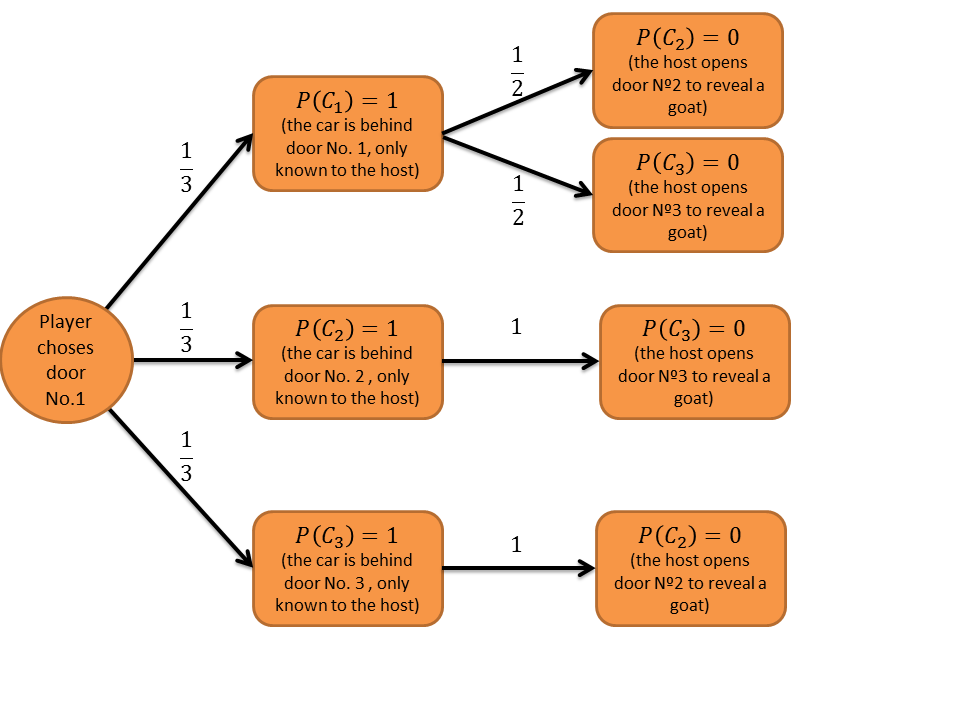
\includegraphics[scale=0.35]{Figures/monty_hall_decision_tree.png}
\caption{Decision tree modelling the Monty Hall problem. }
\label{fig:monty_hall_tree}
\end{figure}

After the player has had her choice, the host will perform an operation on the remaining two doors. The host of the show has complete information of the game, unlike the player.

\begin{equation}
\label{eq:monty_h1}
P(C_{1})=P(C_{1}|\text{\textlnot}C_{2})+P(C_{1}|\text{\textlnot}C_{3})
\end{equation}


\begin{equation}
\label{eq:monty_h2}
P(C_{1})=(\frac{1}{3}\text{\texttimes}\frac{1}{2})+(\frac{1}{3}\text{\texttimes}\frac{1}{2})=1
\end{equation}


\begin{equation}
\label{eq:monty_h3}
P(\text{\textlnot}C_{1})=P(C_{2}|\text{\textlnot}C_{3})+P(C_{3}|\text{\textlnot}C_{2})=(\frac{1}{3}\text{\texttimes}1)+(\frac{1}{3}\text{\texttimes}1)=2/3
\end{equation}

The probability of switching and getting the car is twice \ref{eq:monty_h3} as likely of staying with the first choice and getting the prize\ref{eq:monty_h2}. 


\subsubsection{Quantum Model}

Various Models have been proposed to describe a quantum version of the Monty Hall problem.

[To Introduce more SOURCES]





As the host reveals information, the initial setup is modified. This is an interesting property. Despite being a counter-intuitive problem, a quantum approach to this problem allows an in-depth comparison between the classical measurement and the quantum measurement. The classic Monty Hall problem is modeled using conditional probability and Bayes Rule. In the quantum version, measuring the outcome of the final state yields the result, instead of taking into account the intermediate actions \cite{Fra2011}.

Moreover it is important to realize that there is not a unique way to model a classical problem\cite{Gill2002}. Therefore, when modelling a classical problem, we need to select properties that could potentially benefit from a quantum approch. In \cite{Gill2002} we can observe the attempt to stick as closely to the classical formulation as possible, the host has a system that is correlated to the game system.







